\documentclass[a4paper,11pt]{article}
\usepackage[utf8]{inputenc}
\usepackage[T1]{fontenc}
\usepackage{amsmath,amssymb}
\usepackage[a4paper,left=2cm,right=2cm,top=3.6cm,bottom=2.3cm,headheight=1.1cm,headsep=0.6cm,footskip=1cm]{geometry}
\usepackage{xcolor}
\usepackage{tikz}
\usetikzlibrary{calc,arrows.meta,positioning,shapes.geometric}
\usepackage{fancyhdr}
\usepackage{lastpage}
\usepackage{tabularx}
\usepackage{array}
\usepackage[most]{tcolorbox}
\usepackage{enumitem}
\usepackage{needspace}

% ---------- palet merah dan merah muda ----------
\definecolor{redx}{HTML}{B3202F}
\definecolor{pinkx}{HTML}{E0457B}
\definecolor{maroon}{HTML}{7A1C2C}
\definecolor{softbg}{HTML}{FDF1F4}
\definecolor{salmon}{HTML}{E8836F}
\newcommand{\dis}{\displaystyle}

\setlength{\parindent}{0pt}
\renewcommand{\arraystretch}{1.35}

\tikzset{
  ar/.style={-{Stealth[length=1.8mm]},thick,redx},
  box/.style={draw=redx,thick,rounded corners=3pt,fill=softbg,align=center,inner sep=4pt}
}

% ---------- header berwarna merah ----------
\pagestyle{fancy}
\fancyhf{}
\renewcommand{\headrulewidth}{0pt}
\fancyhead[L]{%
  \begin{tikzpicture}[remember picture,overlay]
    \fill[redx] ([yshift=-1.2cm]current page.north west) rectangle ([yshift=-3.15cm]current page.north east);
    \fill[pinkx] ([yshift=-3.15cm]current page.north west) rectangle ([yshift=-3.25cm]current page.north east);
  \end{tikzpicture}%
  \color{white}\bfseries\large Latihan Soal Lingkaran}
\fancyhead[R]{\color{white}\small Diunduh dari website \textbf{Math1729}\ \,|\,\ 4 Oktober 2026}
\fancyfoot[L]{\small\color{redx}Math1729 --- Lingkaran}
\fancyfoot[R]{\small\color{redx}Halaman \thepage\ dari \pageref{LastPage}}

% ---------- komponen ----------
\newcounter{no}
\newcommand{\bagian}[2]{\par\Needspace{6\baselineskip}\vspace{1.0em}\noindent
  \begin{tcolorbox}[colback=redx,colframe=redx,coltext=white,boxrule=0pt,arc=2pt,left=6pt,right=6pt,top=3pt,bottom=3pt]
  \textbf{#1}\hfill{\small #2}\end{tcolorbox}\setcounter{no}{0}\par\vspace{-0.3em}}
\newcommand{\tingkat}[2]{\par\Needspace{7\baselineskip}\vspace{0.6em}\noindent
  {\color{pinkx}\rule{3pt}{1.1em}}\ {\color{redx}\bfseries #1}\ {\small\color{gray}--- #2}\par\vspace{0.1em}}
\newcommand{\soal}[2]{\par\vspace{0.75em}\stepcounter{no}\noindent
  \begin{minipage}[t]{1.8em}\textbf{\theno.}\end{minipage}%
  \begin{minipage}[t]{\dimexpr\linewidth-1.8em\relax}#1\par\vspace{0.35em}#2\end{minipage}\par}
\newcommand{\poin}[1]{\hfill{\small\color{redx}[#1 poin]}}

% teks di kiri, gambar di kanan
\newcommand{\gbr}[2]{\noindent\begin{minipage}[t]{0.56\linewidth}#1\end{minipage}\hfill\raisebox{\ht\strutbox}{\begin{minipage}[t]{0.41\linewidth}\vspace{0pt}\centering#2\end{minipage}}}

% pilihan jawaban
\newcommand{\pil}[5]{\begin{tabularx}{\linewidth}{@{}*{5}{X}@{}}\textbf{A.}\;#1 & \textbf{B.}\;#2 & \textbf{C.}\;#3 & \textbf{D.}\;#4 & \textbf{E.}\;#5\end{tabularx}}
\newcommand{\pilx}[5]{\begin{tabularx}{\linewidth}{@{}*{3}{X}@{}}\textbf{A.}\;#1 & \textbf{B.}\;#2 & \textbf{C.}\;#3\\[10pt] \textbf{D.}\;#4 & \textbf{E.}\;#5 & \end{tabularx}}
\newcommand{\jwb}{\hfill Jawaban: \rule{4.5cm}{0.4pt}}

\begin{document}
\thispagestyle{fancy}

\begin{center}
  {\color{redx}\fontsize{22}{26}\selectfont\bfseries Latihan Soal Lingkaran\par}
  \vspace{2pt}
  {\color{pinkx}\large Keliling, Luas, Busur, Juring, Sudut, Garis Singgung, dan Persamaan Lingkaran\par}
\end{center}
\vspace{2pt}
\begin{tcolorbox}[colback=softbg,colframe=redx!40,boxrule=0.6pt,arc=3pt,left=8pt,right=8pt,top=5pt,bottom=5pt]
\noindent\textbf{Nama} : \rule{4.6cm}{0.4pt}\hfill\textbf{Kelas} : \rule{2.2cm}{0.4pt}\hfill\textbf{Skor} : \rule{2.2cm}{0.4pt}
\end{tcolorbox}
\vspace{2pt}
\begin{tcolorbox}[colback=white,colframe=pinkx,boxrule=0.8pt,arc=3pt,left=8pt,right=8pt,top=4pt,bottom=4pt,title={\bfseries Petunjuk Pengerjaan},coltitle=white,fonttitle=\small]
\small
\begin{enumerate}[leftmargin=1.4em,itemsep=1pt,topsep=1pt]
\item Soal terdiri atas \textbf{20 pilihan ganda} (5 mudah, 5 sedang, 5 sulit, 5 HOTS), \textbf{5 isian singkat}, dan \textbf{5 uraian (essay)}. Soal disusun berjenjang dari mudah sampai HOTS dan sebagian bergaya UTBK. Alokasi waktu yang disarankan: 120 menit.
\item Skor: pilihan ganda 2 poin, isian singkat 4 poin, uraian 8 poin per soal (total 100 poin). Tidak ada pengurangan skor untuk jawaban salah.
\item Notasi: $O$ pusat lingkaran, $r$ jari-jari, $K$ keliling, dan $L$ luas. Nilai $\pi=\frac{22}{7}$ hanya dipakai jika disebutkan pada soal; jika tidak, tuliskan jawaban dalam bentuk $\pi$. Satuan panjang dalam cm kecuali disebutkan lain. Gambar tidak selalu digambar sesuai skala.
\item Bilangan desimal ditulis dengan tanda koma. Jika perlu, bulatkan hasil sampai dua angka desimal.
\item Kalkulator tidak diperkenankan.
\end{enumerate}
\end{tcolorbox}

% =====================================================================
\bagian{A. Pilihan Ganda}{20 soal $\times$ 2 poin = 40 poin. Pilih satu jawaban yang paling tepat.}

\tingkat{Tingkat Mudah}{soal 1 sampai 5}
\soal{Sebuah taman kota berbentuk lingkaran dengan diameter $28$ m. Lampu hias dipasang mengelilingi tepi taman dengan jarak yang sama, yaitu $4$ m antara dua lampu berurutan. Banyak lampu yang diperlukan adalah \dots\ ($\pi=\frac{22}{7}$).}{\pil{$11$}{$21$}{$22$}{$44$}{$88$}}
\soal{\gbr{Pada gambar, $O$ adalah pusat lingkaran, $\angle AOB=30^\circ$, dan $\angle COD=150^\circ$. Jika luas juring $AOB$ adalah $24$ cm$^2$, luas juring $COD$ adalah \dots\ cm$^2$.}{%
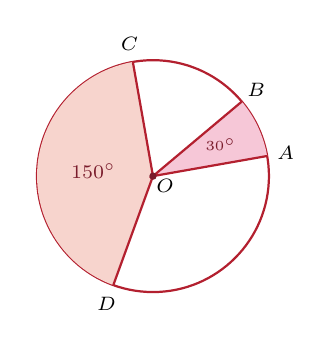
\begin{tikzpicture}[scale=0.95]
\def\R{1.55}
\draw[thick,redx] (0,0) circle (\R);
\fill[pinkx!30] (0,0)--(10:\R) arc (10:40:\R)--cycle;
\fill[salmon!35] (0,0)--(100:\R) arc (100:250:\R)--cycle;
\draw[redx,thick] (10:\R)--(0,0)--(40:\R) (100:\R)--(0,0)--(250:\R);
\fill[maroon] (0,0) circle (1.4pt);
\node[font=\scriptsize,below right,inner sep=1pt] at (0,0) {$O$};
\node[font=\scriptsize] at (10:\R+0.25) {$A$};
\node[font=\scriptsize] at (40:\R+0.25) {$B$};
\node[font=\scriptsize] at (100:\R+0.25) {$C$};
\node[font=\scriptsize] at (250:\R+0.27) {$D$};
\node[font=\tiny,maroon] at (25:1.0) {$30^\circ$};
\node[font=\scriptsize,maroon] at (175:0.8) {$150^\circ$};
\end{tikzpicture}}}{\pil{$48$}{$60$}{$72$}{$96$}{$120$}}
\soal{\gbr{Pada gambar, $AB$ adalah diameter lingkaran berpusat $O$ dan $\angle CAB=38^\circ$. Besar $\angle OCB$ adalah \dots.}{%
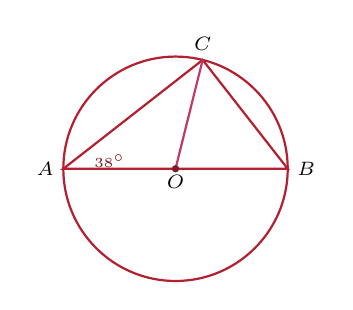
\begin{tikzpicture}[scale=0.95]
\def\R{1.5}
\draw[thick,redx] (0,0) circle (\R);
\coordinate (A) at (180:\R); \coordinate (B) at (0:\R); \coordinate (C) at (76:\R);
\draw[redx,thick] (A)--(B)--(C)--cycle;
\draw[pinkx!85!black,thick] (0,0)--(C);
\fill[maroon] (0,0) circle (1.4pt);
\node[font=\scriptsize,below,inner sep=2pt] at (0,0) {$O$};
\node[font=\scriptsize,left] at (A) {$A$};
\node[font=\scriptsize,right] at (B) {$B$};
\node[font=\scriptsize,above] at (C) {$C$};
\node[font=\tiny,maroon] at ($(A)+(0.62,0.1)$) {$38^\circ$};
\end{tikzpicture}}}{\pil{$38^\circ$}{$52^\circ$}{$64^\circ$}{$76^\circ$}{$90^\circ$}}
\soal{\gbr{Dari titik $P$ di luar lingkaran berpusat $O$ ditarik garis singgung $PA$ dengan $A$ titik singgung. Jika $PA=24$ cm dan $OP=25$ cm, keliling lingkaran tersebut adalah \dots\ cm.}{%
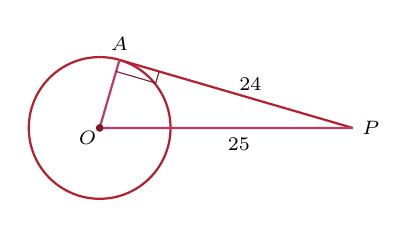
\begin{tikzpicture}
\def\R{0.9}
\coordinate (O) at (0,0); \coordinate (P) at (3.214,0);
\coordinate (A) at (73.74:\R);
\draw[thick,redx] (O) circle (\R);
\draw[redx,thick] (P)--(A);
\draw[pinkx!85!black,thick] (O)--(A) (O)--(P);
\coordinate (u) at ($(A)!0.17!(O)$); \coordinate (v) at ($(A)!0.17!(P)$);
\draw[maroon] (u)--($(u)+(v)-(A)$)--(v);
\fill[maroon] (O) circle (1.4pt);
\node[font=\scriptsize,below left,inner sep=1pt] at (O) {$O$};
\node[font=\scriptsize,right] at (P) {$P$};
\node[font=\scriptsize,above] at (A) {$A$};
\node[font=\scriptsize,above right,inner sep=1pt] at ($(A)!0.5!(P)$) {$24$};
\node[font=\scriptsize,below] at ($(O)!0.55!(P)$) {$25$};
\end{tikzpicture}}}{\pil{$7\pi$}{$10\pi$}{$12\pi$}{$14\pi$}{$25\pi$}}
\soal{Pusat dan jari-jari lingkaran $x^2+y^2-6x+2y-6=0$ berturut-turut adalah \dots.}{\pilx{$(3,-1)$ dan $4$}{$(-3,1)$ dan $4$}{$(3,-1)$ dan $16$}{$(-3,1)$ dan $16$}{$(6,-2)$ dan $4$}}

\tingkat{Tingkat Sedang}{soal 6 sampai 10}
\soal{\gbr{Pada gambar, $AB$ dan $CD$ adalah tali busur sejajar pada lingkaran berjari-jari $10$ cm dengan $AB=16$ cm dan $CD=12$ cm. Kedua tali busur terletak pada sisi yang berbeda terhadap pusat $O$. Jarak antara $AB$ dan $CD$ adalah \dots\ cm.}{%
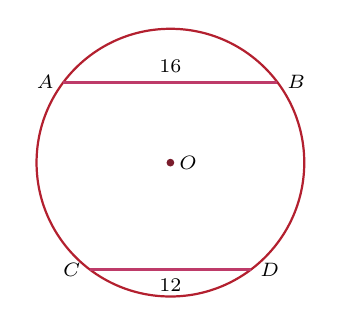
\begin{tikzpicture}
\def\R{1.7}
\draw[thick,redx] (0,0) circle (\R);
\coordinate (A) at (-1.36,1.02); \coordinate (B) at (1.36,1.02);
\coordinate (C) at (-1.02,-1.36); \coordinate (D) at (1.02,-1.36);
\draw[pinkx!85!black,very thick] (A)--(B) (C)--(D);
\fill[maroon] (0,0) circle (1.4pt);
\node[font=\scriptsize,right,inner sep=3pt] at (0,0) {$O$};
\node[font=\scriptsize,left] at (A) {$A$};
\node[font=\scriptsize,right] at (B) {$B$};
\node[font=\scriptsize,left] at (C) {$C$};
\node[font=\scriptsize,right] at (D) {$D$};
\node[font=\scriptsize,above] at (0,1.02) {$16$};
\node[font=\scriptsize,below] at (0,-1.36) {$12$};
\end{tikzpicture}}}{\pil{$2$}{$7$}{$10$}{$14$}{$16$}}
\soal{Sebuah juring lingkaran memiliki keliling $16$ cm dan luas $15$ cm$^2$. Jika sudut pusat juring tersebut kurang dari $\pi$ radian, besar sudut pusatnya adalah \dots\ radian.}{\pil{$\dis\frac35$}{$\dis\frac65$}{$\dis\frac32$}{$\dis\frac53$}{$\dis\frac{10}{3}$}}
\soal{Dua lingkaran berjari-jari $8$ cm dan $2$ cm memiliki jarak kedua pusat $d$. Perhatikan pernyataan berikut.
\begin{enumerate}[label=(\arabic*),leftmargin=1.8em,itemsep=0pt,topsep=2pt]
\item Jika $d=10$ cm, terdapat tepat $3$ garis singgung persekutuan.
\item Jika $d=6$ cm, terdapat tepat $2$ garis singgung persekutuan.
\item Jika $d=26$ cm, panjang garis singgung persekutuan dalamnya adalah $24$ cm.
\item Jika $d=12$ cm, panjang garis singgung persekutuan luarnya adalah $8$ cm.
\end{enumerate}
Pernyataan yang benar adalah \dots.}{\begin{tabularx}{\linewidth}{@{}*{3}{X}@{}}\textbf{A.}\;(1) dan (2) saja & \textbf{B.}\;(2) dan (4) saja & \textbf{C.}\;(1) dan (3) saja\\[3pt] \textbf{D.}\;(1), (3), dan (4) saja & \textbf{E.}\;(2), (3), dan (4) saja & \end{tabularx}}
\soal{Garis $y=x+k$ menyinggung lingkaran $(x-2)^2+(y-1)^2=18$. Selisih nilai $k$ terbesar dan nilai $k$ terkecil yang memenuhi adalah \dots.}{\pil{$2$}{$6$}{$7$}{$10$}{$12$}}
\soal{\gbr{Pada gambar, $ABCD$ adalah segiempat tali busur dengan $\angle DAB=(3x+5)^\circ$, $\angle ABC=(4x+15)^\circ$, dan $\angle BCD=(5x-25)^\circ$. Besar $\angle ADC$ adalah \dots.}{%
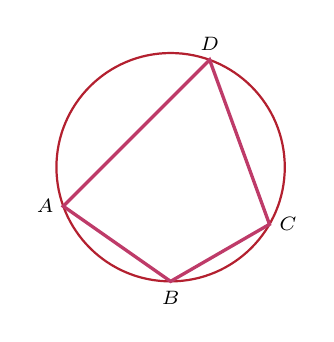
\begin{tikzpicture}
\def\R{1.45}
\draw[thick,redx] (0,0) circle (\R);
\coordinate (A) at (200:\R); \coordinate (B) at (270:\R);
\coordinate (C) at (330:\R); \coordinate (D) at (70:\R);
\draw[pinkx!85!black,very thick] (A)--(B)--(C)--(D)--cycle;
\node[font=\scriptsize,left] at (A) {$A$};
\node[font=\scriptsize,below] at (B) {$B$};
\node[font=\scriptsize,right] at (C) {$C$};
\node[font=\scriptsize,above] at (D) {$D$};
\end{tikzpicture}}}{\pil{$65^\circ$}{$80^\circ$}{$100^\circ$}{$115^\circ$}{$125^\circ$}}

\tingkat{Tingkat Sulit}{soal 11 sampai 15, setara UTBK}
\soal{\gbr{Pada segitiga sama sisi $ABC$ dengan panjang sisi $12$ cm, dibuat tiga lingkaran berjari-jari $6$ cm yang masing-masing berpusat di $A$, $B$, dan $C$. Luas daerah arsiran, yaitu daerah di dalam segitiga yang berada di luar ketiga lingkaran, adalah \dots\ cm$^2$.}{%
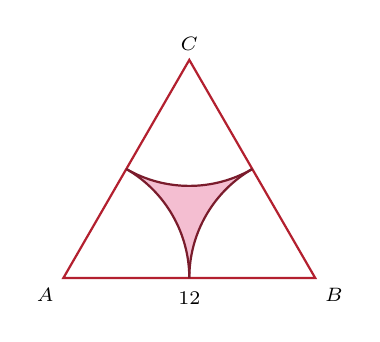
\begin{tikzpicture}
\coordinate (A) at (0,0); \coordinate (B) at (3.2,0); \coordinate (C) at (1.6,2.771);
\fill[pinkx!35] (A)--(B)--(C)--cycle;
\fill[white] (A)--(1.6,0) arc (0:60:1.6)--cycle;
\fill[white] (B)--(1.6,0) arc (180:120:1.6)--cycle;
\fill[white] (C)--($(C)+(240:1.6)$) arc (240:300:1.6)--cycle;
\draw[redx,thick] (A)--(B)--(C)--cycle;
\draw[maroon,thick] (1.6,0) arc (0:60:1.6);
\draw[maroon,thick] (1.6,0) arc (180:120:1.6);
\draw[maroon,thick] ($(C)+(240:1.6)$) arc (240:300:1.6);
\node[font=\scriptsize,below left] at (A) {$A$};
\node[font=\scriptsize,below right] at (B) {$B$};
\node[font=\scriptsize,above] at (C) {$C$};
\node[font=\scriptsize,below] at (1.6,-0.05) {$12$};
\end{tikzpicture}}}{\pil{$18\sqrt3-9\pi$}{$36\sqrt3-18\pi$}{$72\sqrt3-36\pi$}{$36\sqrt3-9\pi$}{$72\sqrt3-18\pi$}}
\soal{\gbr{Sebuah sabuk melilit ketat dua roda yang berjari-jari $10$ cm dan $4$ cm, dengan jarak kedua pusat $12$ cm (lihat gambar). Panjang sabuk tersebut adalah \dots\ cm.}{%
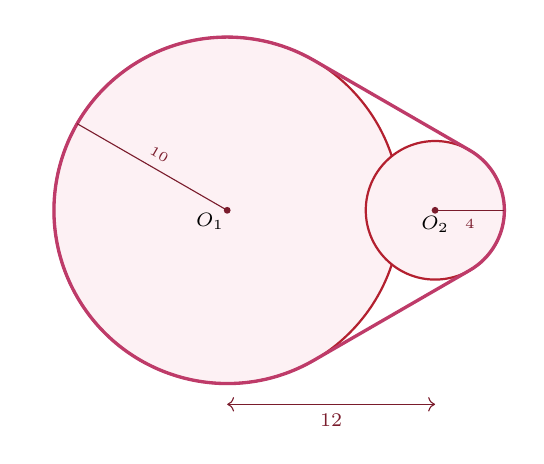
\begin{tikzpicture}[scale=0.88]
\def\R{2.5}\def\r{1.0}\def\d{3.0}
\draw[fill=softbg,draw=redx,thick] (0,0) circle (\R);
\draw[fill=softbg,draw=redx,thick] (\d,0) circle (\r);
\draw[very thick,pinkx!85!black] (60:\R)--($(\d,0)+(60:\r)$) arc (60:-60:\r)--(300:\R) arc (300:60:\R);
\fill[maroon] (0,0) circle (1.4pt) (\d,0) circle (1.4pt);
\node[font=\scriptsize,below left,inner sep=1pt] at (0,0) {$O_1$};
\node[font=\scriptsize,below,inner sep=2pt] at (\d,0) {$O_2$};
\draw[maroon,thin] (0,0)--(150:\R) node[midway,above,sloped,font=\tiny]{$10$};
\draw[maroon,thin] (\d,0)--($(\d,0)+(0:\r)$) node[midway,below,font=\tiny]{$4$};
\draw[<->,maroon] (0,-2.8)--(\d,-2.8) node[midway,below,font=\scriptsize]{$12$};
\end{tikzpicture}}}{\pil{$6\sqrt3+16\pi$}{$12\sqrt3+14\pi$}{$12\sqrt3+16\pi$}{$24\sqrt3+16\pi$}{$12\sqrt3+28\pi$}}
\soal{\gbr{Segitiga $ABC$ siku-siku di $B$. Lingkaran dalam segitiga tersebut menyinggung sisi $AC$ di titik $D$. Jika $AD=3$ cm dan $DC=10$ cm, luas segitiga $ABC$ adalah \dots\ cm$^2$.}{%
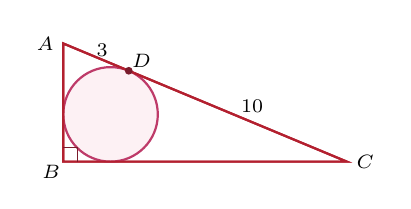
\begin{tikzpicture}
\coordinate (B) at (0,0); \coordinate (C) at (3.6,0); \coordinate (A) at (0,1.5);
\coordinate (D) at ($(A)!0.2308!(C)$);
\draw[redx,thick] (A)--(B)--(C)--cycle;
\draw[pinkx!85!black,thick,fill=softbg] (0.6,0.6) circle (0.6);
\draw[redx,thick] (A)--(B)--(C)--cycle;
\draw[maroon] (0,0.18)--(0.18,0.18)--(0.18,0);
\fill[maroon] (D) circle (1.4pt);
\node[font=\scriptsize,left] at (A) {$A$};
\node[font=\scriptsize,below left,inner sep=1pt] at (B) {$B$};
\node[font=\scriptsize,right] at (C) {$C$};
\node[font=\scriptsize,above right,inner sep=1pt] at (D) {$D$};
\node[font=\scriptsize,above right,inner sep=0pt] at ($(A)!0.5!(D)$) {$3$};
\node[font=\scriptsize,above right,inner sep=1pt] at ($(D)!0.5!(C)$) {$10$};
\end{tikzpicture}}}{\pil{$20$}{$24$}{$28$}{$30$}{$39$}}
\soal{\gbr{Dua lingkaran menyinggung sumbu-$x$ dan sumbu-$y$ sekaligus, serta keduanya melalui titik $(1,2)$. Jarak antara kedua pusat lingkaran tersebut adalah \dots.}{%
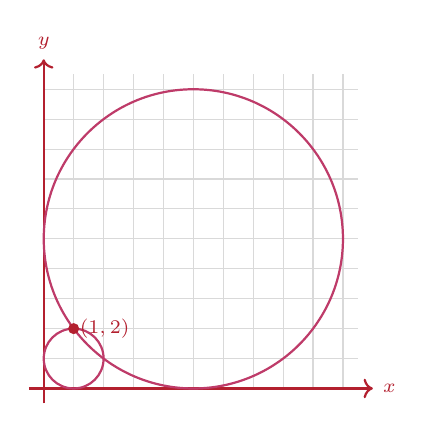
\begin{tikzpicture}[x=0.38cm,y=0.38cm]
\draw[gray!30,xstep=1,ystep=1] (0,0) grid (10.5,10.5);
\draw[->,thick,redx] (-0.5,0)--(11,0) node[right,font=\scriptsize]{$x$};
\draw[->,thick,redx] (0,-0.5)--(0,11) node[above,font=\scriptsize]{$y$};
\draw[pinkx!85!black,thick] (1,1) circle (1);
\draw[pinkx!85!black,thick] (5,5) circle (5);
\fill[redx] (1,2) circle (2pt) node[right,font=\scriptsize,inner sep=2pt]{$(1,2)$};
\end{tikzpicture}}}{\pil{$4\sqrt2$}{$6$}{$8$}{$6\sqrt2$}{$8\sqrt2$}}
\soal{\gbr{Dari titik $P$ di luar lingkaran berpusat $O$ ditarik garis singgung $PA$ dan $PB$ dengan $\angle APB=60^\circ$ dan $PA=6\sqrt3$ cm. Luas daerah arsiran, yaitu daerah yang dibatasi $PA$, $PB$, dan busur minor $AB$, adalah \dots\ cm$^2$.}{%
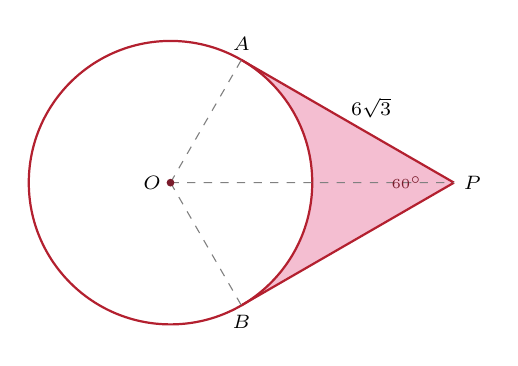
\begin{tikzpicture}
\def\R{1.8}
\coordinate (O) at (0,0); \coordinate (P) at (3.6,0);
\coordinate (A) at (60:\R); \coordinate (B) at (-60:\R);
\fill[pinkx!35] (P)--(A) arc (60:-60:\R)--cycle;
\draw[thick,redx] (O) circle (\R);
\draw[redx,thick] (P)--(A) (P)--(B);
\draw[gray,dashed] (O)--(A) (O)--(B) (O)--(P);
\fill[maroon] (O) circle (1.4pt);
\node[font=\scriptsize,left] at (O) {$O$};
\node[font=\scriptsize,right] at (P) {$P$};
\node[font=\scriptsize,above] at (A) {$A$};
\node[font=\scriptsize,below] at (B) {$B$};
\node[font=\tiny,maroon] at (3.0,0) {$60^\circ$};
\node[font=\scriptsize,above right,inner sep=1pt] at ($(A)!0.5!(P)$) {$6\sqrt3$};
\end{tikzpicture}}}{\pil{$12\pi-18\sqrt3$}{$18\sqrt3-6\pi$}{$36\sqrt3-12\pi$}{$36\sqrt3-6\pi$}{$72\sqrt3-12\pi$}}

\tingkat{Tingkat HOTS}{soal 16 sampai 20, penalaran tingkat tinggi gaya UTBK}
\soal{\gbr{Sebuah koin berjari-jari $2$ cm menggelinding tanpa slip mengelilingi (di luar) sebuah koin tetap berjari-jari $6$ cm sampai kembali ke posisi semula. Selama itu, koin yang menggelinding berputar terhadap pusatnya sendiri sebanyak \dots\ putaran penuh.}{%
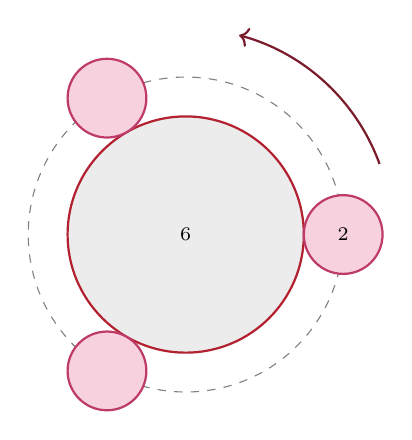
\begin{tikzpicture}
\def\R{1.5}\def\r{0.5}
\draw[fill=gray!15,draw=redx,thick] (0,0) circle (\R);
\node[font=\scriptsize] at (0,0) {$6$};
\draw[dashed,gray] (0,0) circle (\R+\r);
\foreach \a in {0,120,240}{\draw[fill=pinkx!25,draw=pinkx!85!black,thick] (\a:{\R+\r}) circle (\r);}
\node[font=\scriptsize] at (0:2.0) {$2$};
\draw[->,maroon,thick] (20:2.62) arc (20:75:2.62);
\end{tikzpicture}}}{\pil{$3$}{$4$}{$5$}{$6$}{$8$}}
\soal{\gbr{Dua belas titik ditempatkan pada sebuah lingkaran sehingga membagi lingkaran menjadi dua belas busur yang sama panjang. Banyak segitiga siku-siku berbeda yang ketiga titik sudutnya dipilih dari kedua belas titik tersebut adalah \dots.}{%
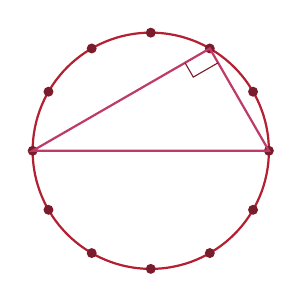
\begin{tikzpicture}
\def\R{1.5}
\draw[thick,redx] (0,0) circle (\R);
\foreach \k in {0,...,11}{\fill[maroon] (30*\k:\R) circle (1.8pt);}
\draw[pinkx!85!black,thick] (0:\R)--(180:\R)--(60:\R)--cycle;
\coordinate (V) at (60:\R);
\coordinate (u) at ($(V)!0.14!(0:\R)$); \coordinate (v) at ($(V)!0.14!(180:\R)$);
\draw[maroon] (u)--($(u)+(v)-(V)$)--(v);
\end{tikzpicture}}}{\pil{$30$}{$36$}{$48$}{$54$}{$60$}}
\soal{\gbr{Pada lingkaran, tali busur $AB=8$ cm tetap, sedangkan titik $P$ bergerak pada busur mayor $AB$ sehingga $\angle APB=30^\circ$ selalu. Luas maksimum segitiga $APB$ adalah \dots\ cm$^2$.}{%
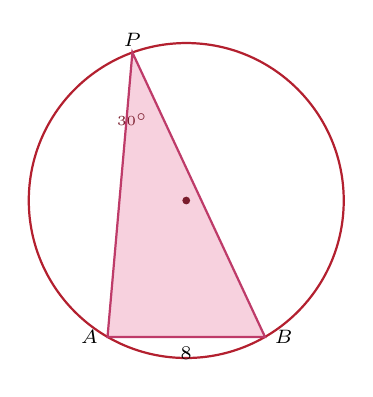
\begin{tikzpicture}
\def\R{2.0}
\coordinate (A) at (240:\R); \coordinate (B) at (300:\R); \coordinate (P) at (110:\R);
\fill[pinkx!25] (A)--(B)--(P)--cycle;
\draw[thick,redx] (0,0) circle (\R);
\draw[pinkx!85!black,thick] (A)--(B)--(P)--cycle;
\fill[maroon] (0,0) circle (1.4pt);
\node[font=\scriptsize,left] at (A) {$A$};
\node[font=\scriptsize,right] at (B) {$B$};
\node[font=\scriptsize,above,inner sep=2pt] at (P) {$P$};
\node[font=\scriptsize,below] at (0,-1.732) {$8$};
\node[font=\tiny,maroon] at ($(P)+(0.0,-0.85)$) {$30^\circ$};
\end{tikzpicture}}}{\pil{$16+8\sqrt3$}{$32+8\sqrt3$}{$24+16\sqrt3$}{$32+16\sqrt3$}{$64+16\sqrt3$}}
\soal{Diketahui titik $A(-3,0)$ dan $B(3,0)$. Himpunan semua titik $P(x,y)$ yang memenuhi $PA=2\,PB$ membentuk sebuah lingkaran. Luas daerah yang dibatasi lingkaran tersebut adalah \dots.}{\pil{$4\pi$}{$8\pi$}{$9\pi$}{$12\pi$}{$16\pi$}}
\soal{Berapakah luas daerah tembereng yang dibatasi tali busur $AB$ dan busur minor $AB$ pada lingkaran berpusat $O$?
\begin{enumerate}[label=(\arabic*),leftmargin=1.8em,itemsep=0pt,topsep=2pt]
\item Jari-jari lingkaran adalah $12$ cm.
\item Jarak $O$ ke tali busur $AB$ adalah $6$ cm.
\end{enumerate}}{\begin{tabularx}{\linewidth}{@{}lX@{}}
\textbf{A.} & Pernyataan (1) SAJA cukup untuk menjawab pertanyaan, tetapi pernyataan (2) SAJA tidak cukup.\\
\textbf{B.} & Pernyataan (2) SAJA cukup untuk menjawab pertanyaan, tetapi pernyataan (1) SAJA tidak cukup.\\
\textbf{C.} & DUA pernyataan BERSAMA-SAMA cukup untuk menjawab pertanyaan, tetapi SATU pernyataan SAJA tidak cukup.\\
\textbf{D.} & Pernyataan (1) SAJA cukup dan pernyataan (2) SAJA cukup untuk menjawab pertanyaan.\\
\textbf{E.} & Pernyataan (1) dan pernyataan (2) tidak cukup untuk menjawab pertanyaan.
\end{tabularx}}

% =====================================================================
\bagian{B. Isian Singkat}{5 soal $\times$ 4 poin = 20 poin. Tuliskan hanya jawaban akhir.}

\tingkat{Tingkat Sedang}{soal 1 dan 2}
\soal{\gbr{Pada gambar, $O$ adalah pusat lingkaran berjari-jari $10$ cm dan $\angle AOB=90^\circ$. Luas daerah arsiran (tembereng) adalah \dots\ cm$^2$ (tuliskan dalam bentuk $\pi$).}{%
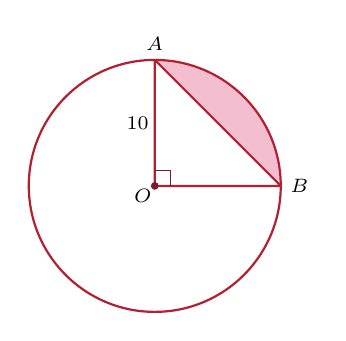
\begin{tikzpicture}
\def\R{1.6}
\fill[pinkx!35] (0,\R) arc (90:0:\R)--cycle;
\draw[thick,redx] (0,0) circle (\R);
\draw[redx,thick] (0,0)--(0,\R) (0,0)--(\R,0) (0,\R)--(\R,0);
\fill[maroon] (0,0) circle (1.4pt);
\draw[maroon] (0,0.2)--(0.2,0.2)--(0.2,0);
\node[font=\scriptsize,below left,inner sep=1pt] at (0,0) {$O$};
\node[font=\scriptsize,above] at (0,\R) {$A$};
\node[font=\scriptsize,right] at (\R,0) {$B$};
\node[font=\scriptsize,left,inner sep=2pt] at (0,0.8) {$10$};
\end{tikzpicture}}}{\jwb}
\soal{\gbr{Segienam beraturan dengan panjang sisi $6$ cm digambar bersama lingkaran luarnya dan lingkaran dalamnya. Luas daerah arsiran di antara kedua lingkaran tersebut adalah \dots\ cm$^2$ (tuliskan dalam bentuk $\pi$).}{%
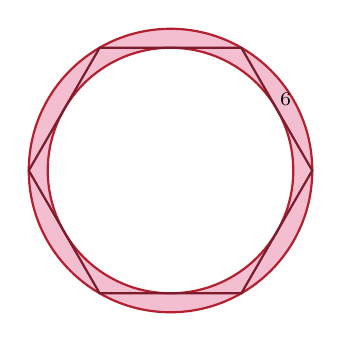
\begin{tikzpicture}
\def\R{1.8}\def\rr{1.559}
\fill[pinkx!35,even odd rule] (0,0) circle (\R) (0,0) circle (\rr);
\draw[thick,redx] (0,0) circle (\R);
\draw[thick,redx] (0,0) circle (\rr);
\draw[maroon,thick] (0:\R)--(60:\R)--(120:\R)--(180:\R)--(240:\R)--(300:\R)--cycle;
\node[font=\scriptsize,above right,inner sep=1pt] at ($(0:\R)!0.5!(60:\R)$) {$6$};
\end{tikzpicture}}}{\jwb}

\tingkat{Tingkat Sulit}{soal 3 sampai 5}
\soal{\gbr{Tiga lingkaran berjari-jari $3$ cm, $4$ cm, dan $5$ cm saling bersinggungan di luar (lihat gambar). Luas segitiga yang titik-titik sudutnya adalah pusat ketiga lingkaran tersebut adalah \dots\ cm$^2$.}{%
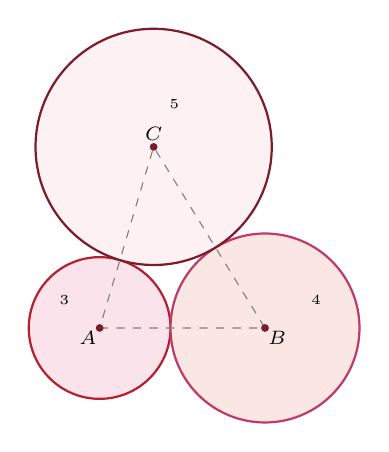
\begin{tikzpicture}
\coordinate (A) at (0,0); \coordinate (B) at (2.1,0); \coordinate (C) at (0.6857,2.30);
\draw[thick,redx,fill=pinkx!15] (A) circle (0.9);
\draw[thick,pinkx!85!black,fill=salmon!20] (B) circle (1.2);
\draw[thick,maroon,fill=softbg] (C) circle (1.5);
\draw[gray,dashed] (A)--(B)--(C)--cycle;
\fill[maroon] (A) circle (1.4pt) (B) circle (1.4pt) (C) circle (1.4pt);
\node[font=\scriptsize,below left,inner sep=1pt] at (A) {$A$};
\node[font=\scriptsize,below right,inner sep=1pt] at (B) {$B$};
\node[font=\scriptsize,above,inner sep=2pt] at (C) {$C$};
\node[font=\tiny] at (-0.45,0.35) {$3$};
\node[font=\tiny] at (2.75,0.35) {$4$};
\node[font=\tiny] at (0.95,2.85) {$5$};
\end{tikzpicture}}}{\jwb}
\soal{\gbr{Titik $T(6,2)$ terletak pada lingkaran $x^2+y^2-6x+4y-12=0$. Garis singgung lingkaran di titik $T$ bersama sumbu-$x$ dan sumbu-$y$ membatasi sebuah segitiga (daerah arsiran). Luas segitiga tersebut adalah \dots\ satuan luas.}{%
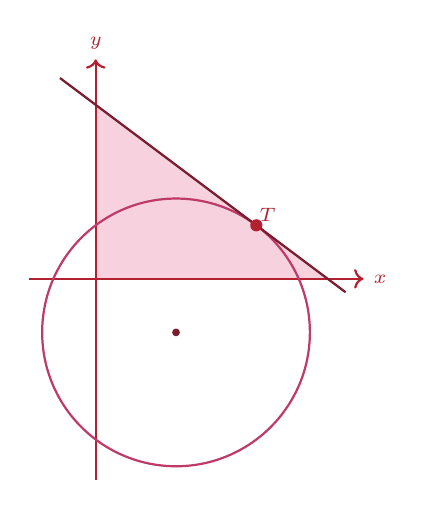
\begin{tikzpicture}[x=0.34cm,y=0.34cm]
\fill[pinkx!25] (0,0)--(8.667,0)--(0,6.5)--cycle;
\draw[->,thick,redx] (-2.5,0)--(10,0) node[right,font=\scriptsize]{$x$};
\draw[->,thick,redx] (0,-7.5)--(0,8.2) node[above,font=\scriptsize]{$y$};
\draw[pinkx!85!black,thick] (3,-2) circle (5);
\draw[maroon,thick] (-1.333,7.5)--(9.333,-0.5);
\fill[redx] (6,2) circle (2.2pt) node[above right,font=\scriptsize,inner sep=1pt]{$T$};
\fill[maroon] (3,-2) circle (1.4pt);
\end{tikzpicture}}}{\jwb}
\soal{\gbr{Gambar menunjukkan tiga setengah lingkaran dengan diameter $AB$, $AC$, dan $CB$, dengan $C$ terletak pada $AB$, $AC=8$ cm, dan $CB=20$ cm. Luas daerah arsiran adalah \dots\ cm$^2$ (tuliskan dalam bentuk $\pi$).}{%
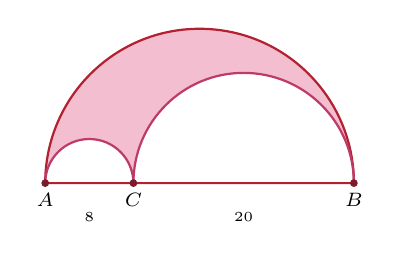
\begin{tikzpicture}
\fill[pinkx!35,even odd rule] (0,0) arc (180:0:1.96)--cycle (0,0) arc (180:0:0.56)--cycle (1.12,0) arc (180:0:1.4)--cycle;
\draw[redx,thick] (0,0) arc (180:0:1.96)--cycle;
\draw[pinkx!85!black,thick] (0,0) arc (180:0:0.56);
\draw[pinkx!85!black,thick] (1.12,0) arc (180:0:1.4);
\fill[maroon] (0,0) circle (1.4pt) (1.12,0) circle (1.4pt) (3.92,0) circle (1.4pt);
\node[font=\scriptsize,below] at (0,0) {$A$};
\node[font=\scriptsize,below] at (1.12,0) {$C$};
\node[font=\scriptsize,below] at (3.92,0) {$B$};
\node[font=\tiny,below] at (0.56,-0.25) {$8$};
\node[font=\tiny,below] at (2.52,-0.25) {$20$};
\end{tikzpicture}}}{\jwb}

% =====================================================================
\Needspace{16\baselineskip}
\bagian{C. Uraian (Essay)}{5 soal $\times$ 8 poin = 40 poin. Tuliskan langkah penyelesaian dengan lengkap.}

\tingkat{Tingkat Sedang}{soal 1 dan 2}
\soal{\gbr{Sebuah wiper kaca depan bus berputar pada poros $O$. Bilah wiper terpasang mulai dari jarak $15$ cm sampai $60$ cm dari poros, dan menyapu kaca dengan sudut sapuan $120^\circ$ (daerah arsiran pada gambar).\par\smallskip
(a) Tentukan luas kaca yang disapu bilah wiper.\par
(b) Tentukan panjang lintasan ujung bilah yang terjauh dan yang terdekat dari poros.\par
(c) Tentukan keliling daerah yang disapu.\par
(d) Jika sudut sapuan diubah menjadi $150^\circ$, berapa persen luas sapuan bertambah?}{%
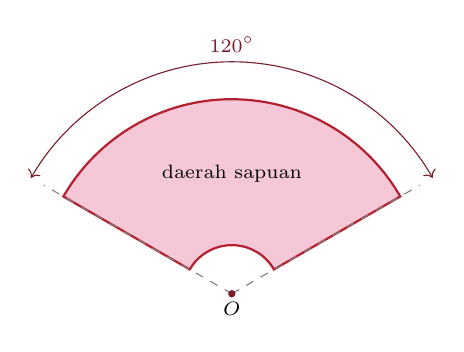
\begin{tikzpicture}[scale=0.95]
\fill[pinkx!30] (30:2.6) arc (30:150:2.6)--(150:0.65) arc (150:30:0.65)--cycle;
\draw[redx,thick] (30:2.6) arc (30:150:2.6)--(150:0.65) arc (150:30:0.65)--cycle;
\draw[gray,dashed] (0,0)--(30:2.9) (0,0)--(150:2.9);
\fill[maroon] (0,0) circle (1.4pt);
\node[font=\scriptsize,below,inner sep=3pt] at (0,0) {$O$};
\draw[<->,maroon,thin] (30:3.1) arc (30:150:3.1);
\node[font=\scriptsize,maroon,above] at (90:3.1) {$120^\circ$};
\node[font=\scriptsize] at (90:1.6) {daerah sapuan};
\end{tikzpicture}}}{\poin{8}}
\soal{Sebuah lingkaran melalui tiga titik $A(8,2)$, $B(0,6)$, dan $C(6,-2)$.\par\smallskip
(a) Tentukan persamaan lingkaran tersebut dalam bentuk umum $x^2+y^2+Dx+Ey+F=0$.\par
(b) Ubah ke bentuk baku, lalu tentukan pusat dan jari-jarinya.\par
(c) Tentukan posisi titik $(7,5)$ dan titik $(9,6)$ terhadap lingkaran (di dalam, pada, atau di luar lingkaran).\par
(d) Tentukan persamaan garis singgung lingkaran di titik $(7,5)$, dan panjang garis singgung dari titik $(9,6)$ ke lingkaran.}{\poin{8}}

\tingkat{Tingkat Sulit}{soal 3 dan 4}
\soal{\gbr{Dua lingkaran berjari-jari $6$ cm berpusat di $O_1$ dan $O_2$ dengan $O_1O_2=6$ cm, sehingga keduanya berpotongan di titik $A$ dan $B$. Daerah irisan kedua lingkaran diarsir.\par\smallskip
(a) Buktikan bahwa $\angle AO_1B=120^\circ$.\par
(b) Tentukan panjang tali busur $AB$.\par
(c) Tentukan luas tembereng pada lingkaran berpusat $O_1$ yang dibatasi tali busur $AB$.\par
(d) Tentukan luas dan keliling daerah irisan tersebut.}{%
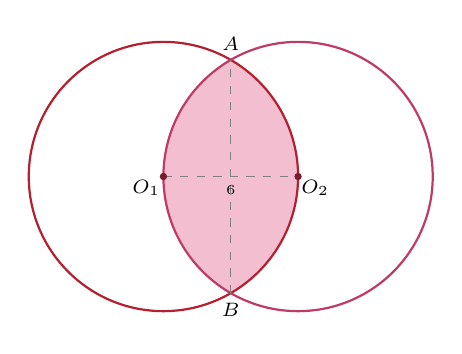
\begin{tikzpicture}[scale=0.95]
\def\R{1.8}
\begin{scope}
\clip (0,0) circle (\R);
\fill[pinkx!35] (\R,0) circle (\R);
\end{scope}
\draw[thick,redx] (0,0) circle (\R);
\draw[thick,pinkx!85!black] (\R,0) circle (\R);
\draw[gray,dashed] (0.9,-1.5588)--(0.9,1.5588);
\draw[gray,dashed] (0,0)--(\R,0);
\fill[maroon] (0,0) circle (1.4pt) (\R,0) circle (1.4pt);
\node[font=\scriptsize,below left,inner sep=1pt] at (0,0) {$O_1$};
\node[font=\scriptsize,below right,inner sep=1pt] at (\R,0) {$O_2$};
\node[font=\scriptsize,above] at (0.9,1.5588) {$A$};
\node[font=\scriptsize,below] at (0.9,-1.5588) {$B$};
\node[font=\tiny] at (0.9,-0.18) {$6$};
\end{tikzpicture}}}{\poin{8}}
\soal{\gbr{Sebuah topi pesta berbentuk kerucut dibuat dengan menggulung selembar kertas berbentuk juring lingkaran berjari-jari $20$ cm dan sudut pusat $216^\circ$ (tanpa tumpang tindih).\par\smallskip
(a) Tentukan panjang busur juring, lalu tentukan jari-jari alas topi.\par
(b) Tentukan tinggi dan volume topi.\par
(c) Tentukan luas kertas yang dipakai, dan buktikan bahwa nilainya sama dengan $\pi\cdot r\cdot s$ dengan $r$ jari-jari alas dan $s$ garis pelukis kerucut.\par
(d) Dari satu lembar kertas berbentuk lingkaran penuh berjari-jari $20$ cm, juring $216^\circ$ dipakai untuk topi pertama dan juring sisanya untuk topi kedua. Buktikan bahwa jumlah jari-jari alas kedua topi sama dengan $20$ cm.}{%
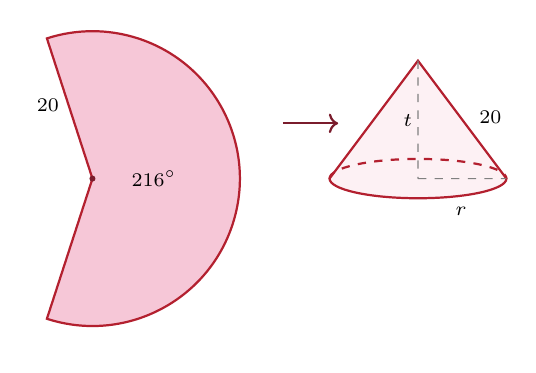
\begin{tikzpicture}[scale=0.78]
\fill[pinkx!30] (0,0)--(-108:2.4) arc (-108:108:2.4)--cycle;
\draw[redx,thick] (0,0)--(-108:2.4) arc (-108:108:2.4)--cycle;
\fill[maroon] (0,0) circle (1.4pt);
\node[font=\scriptsize] at (0:1.0) {$216^\circ$};
\node[font=\scriptsize,left] at (108:1.25) {$20$};
\draw[->,thick,maroon] (3.1,0.9)--(4.0,0.9);
\coordinate (T) at (5.3,1.92);
\draw[redx,thick,fill=softbg] (T)--(3.86,0) arc (180:360:1.44 and 0.32)--cycle;
\draw[redx,thick,dashed] (3.86,0) arc (180:0:1.44 and 0.32);
\draw[gray,dashed] (T)--(5.3,0) (5.3,0)--(6.74,0);
\node[font=\scriptsize,right,inner sep=2pt] at (6.2,1.0) {$20$};
\node[font=\scriptsize,below] at (6.0,-0.3) {$r$};
\node[font=\scriptsize,left,inner sep=2pt] at (5.3,0.95) {$t$};
\end{tikzpicture}}}{\poin{8}}

\tingkat{Tingkat HOTS}{soal 5}
\soal{\gbr{Pada bidang koordinat (satuan meter), dua tiang gawang berada di $A(0,3)$ dan $B(0,9)$. Seorang pemain berlari sepanjang sumbu-$x$ positif dan, di setiap titik $P(x,0)$, melihat gawang dengan sudut tembak $\angle APB$. Pelatih ingin mengetahui posisi $P$ yang memberi sudut tembak terbesar.\par\smallskip
(a) Pusat setiap lingkaran yang melalui $A$ dan $B$ terletak pada sebuah garis. Tentukan persamaan garis itu.\par
(b) Tentukan pusat dan jari-jari lingkaran yang melalui $A$ dan $B$ serta menyinggung sumbu-$x$ positif di titik $T$. Tentukan koordinat $T$.\par
(c) Hitunglah $\angle ATB$.\par
(d) Misalkan $P'$ titik lain pada sumbu-$x$ positif. Jelaskan mengapa $\angle AP'B<\angle ATB$. (Petunjuk: ruas $P'A$ memotong lingkaran di titik $Q$; gunakan sudut luar segitiga.) Simpulkan posisi dan besar sudut tembak maksimum.}{%
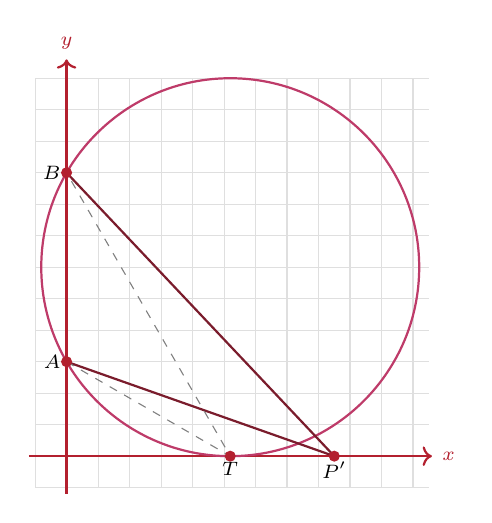
\begin{tikzpicture}[x=0.4cm,y=0.4cm]
\draw[gray!25,xstep=1,ystep=1] (-1,-1) grid (11.5,12);
\draw[->,thick,redx] (-1.2,0)--(11.6,0) node[right,font=\scriptsize]{$x$};
\draw[->,thick,redx] (0,-1.2)--(0,12.6) node[above,font=\scriptsize]{$y$};
\draw[pinkx!85!black,thick] (5.196,6) circle (6);
\coordinate (A) at (0,3); \coordinate (B) at (0,9); \coordinate (T) at (5.196,0); \coordinate (Pp) at (8.5,0);
\draw[maroon,thick] (A)--(Pp)--(B);
\draw[gray,dashed] (A)--(T)--(B);
\fill[redx] (A) circle (2pt) (B) circle (2pt) (T) circle (2pt) (Pp) circle (2pt);
\node[font=\scriptsize,left,inner sep=2pt] at (A) {$A$};
\node[font=\scriptsize,left,inner sep=2pt] at (B) {$B$};
\node[font=\scriptsize,below,inner sep=2pt] at (T) {$T$};
\node[font=\scriptsize,below,inner sep=2pt] at (Pp) {$P'$};
\end{tikzpicture}}}{\poin{8}}

% =====================================================================
\newpage
\bagian{Kunci Jawaban dan Pembahasan Singkat}{Untuk guru dan pembahasan mandiri}
\par\vspace{0.6em}{\bfseries\color{redx}Kunci Pilihan Ganda}\par\vspace{0.3em}
\small
\begin{tabularx}{\linewidth}{@{}*{10}{>{\centering\arraybackslash}X}@{}}\hline \textbf{1} & \textbf{2} & \textbf{3} & \textbf{4} & \textbf{5} & \textbf{6} & \textbf{7} & \textbf{8} & \textbf{9} & \textbf{10}\\ \hline C & E & B & D & A & D & B & C & E & A\\ \hline\end{tabularx}\\[6pt]
\begin{tabularx}{\linewidth}{@{}*{10}{>{\centering\arraybackslash}X}@{}}\hline \textbf{11} & \textbf{12} & \textbf{13} & \textbf{14} & \textbf{15} & \textbf{16} & \textbf{17} & \textbf{18} & \textbf{19} & \textbf{20}\\ \hline B & C & D & A & C & B & E & D & E & C\\ \hline\end{tabularx}
\par\vspace{0.8em}{\bfseries\color{redx}\normalsize Pembahasan Pilihan Ganda}\par\vspace{0.2em}
\small\begin{enumerate}[leftmargin=2em,itemsep=2pt,topsep=2pt]
\item[\textbf{1.}] \textbf{(C)} Keliling taman $K=\pi d=\dis\frac{22}{7}\cdot28=88$ m. Banyak lampu $=\dis\frac{88}{4}=22$. (Jebakan: $88$ adalah keliling taman, bukan banyak lampu.)
\item[\textbf{2.}] \textbf{(E)} Pada lingkaran yang sama, luas juring sebanding dengan sudut pusatnya: $\dis\frac{L_{COD}}{L_{AOB}}=\frac{150^\circ}{30^\circ}=5$, sehingga $L_{COD}=5\times24=120$ cm$^2$.
\item[\textbf{3.}] \textbf{(B)} $AB$ diameter, sehingga $\angle ACB=90^\circ$ (sudut keliling yang menghadap diameter). Pada $\triangle ABC$: $\angle ABC=180^\circ-90^\circ-38^\circ=52^\circ$. Karena $OB=OC$ (jari-jari), $\triangle OBC$ sama kaki dan $\angle OCB=\angle OBC=52^\circ$. (Jebakan: $38^\circ$ adalah $\angle OCA$ dan $76^\circ$ adalah $\angle BOC$.)
\item[\textbf{4.}] \textbf{(D)} Jari-jari $OA$ tegak lurus garis singgung $PA$, sehingga $\triangle OAP$ siku-siku di $A$ dan $OA=\sqrt{25^2-24^2}=\sqrt{49}=7$. Keliling $=2\pi\cdot7=14\pi$ cm.
\item[\textbf{5.}] \textbf{(A)} Lengkapkan kuadrat: $(x-3)^2+(y+1)^2=6+9+1=16$. Pusat $(3,-1)$ dan jari-jari $\sqrt{16}=4$. (Jebakan C dan D: $16$ adalah $r^2$, bukan $r$.)
\item[\textbf{6.}] \textbf{(D)} Jarak tali busur $AB$ ke pusat: $\sqrt{10^2-8^2}=6$. Jarak tali busur $CD$ ke pusat: $\sqrt{10^2-6^2}=8$. Karena berada di sisi berbeda, jarak keduanya $6+8=14$ cm. (Jebakan $2$: jika kedua tali busur berada di sisi yang sama.)
\item[\textbf{7.}] \textbf{(B)} Keliling juring $2r+s=16$ dan luas $\frac12rs=15$. Substitusi $s=16-2r$: $r(16-2r)=30\Rightarrow r^2-8r+15=0\Rightarrow r=3$ atau $r=5$. Untuk $r=3$: $s=10$ dan $\theta=\frac{10}{3}\approx3{,}33>\pi$ (ditolak). Untuk $r=5$: $s=6$ dan $\theta=\dis\frac{s}{r}=\frac65<\pi$ (memenuhi).
\item[\textbf{8.}] \textbf{(C)} (1) \emph{Benar}: $d=10=8+2$, kedua lingkaran bersinggungan luar, sehingga ada $3$ garis singgung persekutuan. (2) \emph{Salah}: $d=6=8-2$, bersinggungan dalam, hanya $1$ garis singgung persekutuan. (3) \emph{Benar}: $\sqrt{26^2-(8+2)^2}=\sqrt{576}=24$. (4) \emph{Salah}: $\sqrt{12^2-(8-2)^2}=\sqrt{108}=6\sqrt3\approx10{,}4$, bukan $8$.
\item[\textbf{9.}] \textbf{(E)} Jarak pusat $(2,1)$ ke garis $x-y+k=0$ harus sama dengan jari-jari $\sqrt{18}=3\sqrt2$: $\dis\frac{|2-1+k|}{\sqrt2}=3\sqrt2\Rightarrow|k+1|=6$. Jadi $k=5$ atau $k=-7$, dan selisihnya $5-(-7)=12$.
\item[\textbf{10.}] \textbf{(A)} Sudut berhadapan segiempat tali busur berjumlah $180^\circ$: $\angle DAB+\angle BCD=(3x+5)+(5x-25)=180\Rightarrow x=25$. Maka $\angle ABC=4(25)+15=115^\circ$ dan $\angle ADC=180^\circ-115^\circ=65^\circ$. (Jebakan: $115^\circ$ adalah $\angle ABC$.)
\item[\textbf{11.}] \textbf{(B)} Luas segitiga sama sisi sisi $12$: $\frac{\sqrt3}{4}\cdot144=36\sqrt3$. Ketiga juring masing-masing bersudut $60^\circ$ dan berjari-jari $6$, sehingga jumlah luasnya $3\cdot\frac16\pi\cdot36=18\pi$ (setara setengah lingkaran). Luas arsiran $=36\sqrt3-18\pi$ (sekitar $5{,}8$ cm$^2$).
\item[\textbf{12.}] \textbf{(C)} Panjang sabuk $=$ dua garis singgung persekutuan luar $+$ dua busur. Garis singgung: $\sqrt{12^2-(10-4)^2}=6\sqrt3$, jadi dua garis $=12\sqrt3$. Sudut $\alpha$ antara garis pusat dan jari-jari ke titik singgung memenuhi $\cos\alpha=\dis\frac{10-4}{12}=\frac12$, sehingga $\alpha=60^\circ$. Busur pada roda besar $=360^\circ-2\cdot60^\circ=240^\circ$: $\frac{240}{360}\cdot2\pi\cdot10=\frac{40\pi}{3}$. Busur pada roda kecil $=2\cdot60^\circ=120^\circ$: $\frac{120}{360}\cdot2\pi\cdot4=\frac{8\pi}{3}$. Jumlah busur $=\frac{48\pi}{3}=16\pi$. Panjang sabuk $=12\sqrt3+16\pi$. (Jebakan B: memakai $180^\circ$ untuk kedua busur, hasilnya $12\sqrt3+14\pi$.)
\item[\textbf{13.}] \textbf{(D)} Panjang garis singgung dari satu titik ke lingkaran sama: $AF=AD=3$ dan $CE=CD=10$, sehingga $AC=13$. Misalkan jari-jari lingkaran dalam $r$; karena siku-siku di $B$, $BF=BE=r$. Maka $AB=3+r$ dan $BC=10+r$. Pythagoras: $(3+r)^2+(10+r)^2=13^2\Rightarrow r^2+13r-30=0\Rightarrow(r+15)(r-2)=0$, sehingga $r=2$. Sisi $AB=5$, $BC=12$, dan luas $=\frac12\cdot5\cdot12=30$ cm$^2$.
\item[\textbf{14.}] \textbf{(A)} Lingkaran yang menyinggung kedua sumbu dan melalui $(1,2)$ (kuadran I) berpusat di $(r,r)$ dengan jari-jari $r$. Syarat: $(1-r)^2+(2-r)^2=r^2\Rightarrow r^2-6r+5=0\Rightarrow r=1$ atau $r=5$. Pusatnya $(1,1)$ dan $(5,5)$, dengan jarak $\sqrt{4^2+4^2}=4\sqrt2$.
\item[\textbf{15.}] \textbf{(C)} $OP$ membagi dua $\angle APB$, sehingga $\angle APO=30^\circ$. Pada $\triangle OAP$ siku-siku di $A$: $OA=PA\tan30^\circ=6\sqrt3\cdot\frac{1}{\sqrt3}=6$. Luas layang-layang $OAPB=2\cdot\frac12\cdot6\cdot6\sqrt3=36\sqrt3$. Sudut $\angle AOB=360^\circ-90^\circ-90^\circ-60^\circ=120^\circ$, sehingga luas juring $AOB=\frac13\pi\cdot36=12\pi$. Luas arsiran $=36\sqrt3-12\pi$.
\item[\textbf{16.}] \textbf{(B)} Pusat koin yang menggelinding bergerak pada lingkaran berjari-jari $6+2=8$ cm, dengan panjang lintasan $2\pi\cdot8=16\pi$. Koin berputar satu kali setiap menempuh $2\pi\cdot2=4\pi$. Banyak putaran $=\dis\frac{16\pi}{4\pi}=4$, yaitu $\dis\frac{R+r}{r}$. (Jebakan $3$: memakai $\frac{R}{r}$ saja.)
\item[\textbf{17.}] \textbf{(E)} Segitiga yang titik sudutnya pada lingkaran siku-siku jika dan hanya jika sisi miringnya diameter (kebalikan teorema sudut keliling pada diameter). Dari $12$ titik terdapat $6$ diameter. Untuk setiap diameter, titik sudut siku-sikunya dapat dipilih dari $10$ titik lain. Banyaknya $=6\times10=60$. Tidak ada hitungan ganda karena setiap segitiga siku-siku hanya memiliki satu sisi miring. (Jebakan $120$: menghitung $12\times10$ sehingga tiap diameter terhitung dua kali.)
\item[\textbf{18.}] \textbf{(D)} Jari-jari lingkaran luar: $AB=2R\sin30^\circ\Rightarrow R=\dis\frac{8}{2\cdot\frac12}=8$. Jarak pusat ke $AB$ adalah $\sqrt{8^2-4^2}=4\sqrt3$. Karena $30^\circ<90^\circ$, $P$ berada di sisi yang sama dengan pusat. Tinggi terbesar tercapai bila $P$ tepat di atas pusat pada sumbu simetri, yaitu $8+4\sqrt3$. Luas maksimum $=\frac12\cdot8\cdot(8+4\sqrt3)=32+16\sqrt3$.
\item[\textbf{19.}] \textbf{(E)} $PA=2PB\Rightarrow(x+3)^2+y^2=4\big[(x-3)^2+y^2\big]\Rightarrow3x^2-30x+3y^2+27=0\Rightarrow x^2-10x+y^2+9=0$, yaitu $(x-5)^2+y^2=16$. Jari-jari $4$, luas $=16\pi$. (Cek: titik $(1,0)$ memberi $PA=4$ dan $PB=2$.)
\item[\textbf{20.}] \textbf{(C)} Pernyataan (1) saja hanya memberi $r$, sedangkan besar sudut pusat belum diketahui. Pernyataan (2) saja hanya memberi jarak tanpa $r$. Gabungan: $\cos\frac{\angle AOB}{2}=\dis\frac{6}{12}\Rightarrow\frac{\angle AOB}{2}=60^\circ$, sehingga $\angle AOB=120^\circ$ dan luas tembereng $=\frac13\pi\cdot144-\frac12\cdot144\sin120^\circ=48\pi-36\sqrt3$. Jadi keduanya diperlukan bersama-sama.
\end{enumerate}
\par\Needspace{6\baselineskip}\vspace{0.6em}{\bfseries\color{redx}\normalsize Pembahasan Isian Singkat}\par\vspace{0.2em}
\small\begin{enumerate}[leftmargin=2em,itemsep=2pt,topsep=2pt]
\item[\textbf{1.}] \textbf{Jawaban: $25\pi-50$.} Tembereng $=$ juring $-$ segitiga $=\frac14\pi\cdot10^2-\frac12\cdot10\cdot10=25\pi-50$ cm$^2$.
\item[\textbf{2.}] \textbf{Jawaban: $9\pi$.} Jari-jari lingkaran luar $R=6$ (sama dengan sisi segienam beraturan) dan jari-jari lingkaran dalam $r=3\sqrt3$. Luas cincin $=\pi(R^2-r^2)=\pi(36-27)=9\pi$. Perhatikan $R^2-r^2=\left(\frac{\text{sisi}}{2}\right)^2$ sehingga luas cincin selalu $\pi\left(\frac{6}{2}\right)^2$.
\item[\textbf{3.}] \textbf{Jawaban: $12\sqrt5$.} Sisi segitiga pusat adalah jumlah dua jari-jari: $3+4=7$, $3+5=8$, dan $4+5=9$. Setengah keliling $s=12$. Rumus Heron: $L=\sqrt{12\cdot5\cdot4\cdot3}=\sqrt{720}=12\sqrt5$.
\item[\textbf{4.}] \textbf{Jawaban: $\dis\frac{169}{6}$.} Bentuk baku: $(x-3)^2+(y+2)^2=25$, pusat $(3,-2)$. Garis singgung di $(6,2)$: $(6-3)(x-3)+(2+2)(y+2)=25\Rightarrow3x+4y=26$. Titik potong sumbu: $\left(\frac{26}{3},0\right)$ dan $\left(0,\frac{13}{2}\right)$. Luas $=\frac12\cdot\frac{26}{3}\cdot\frac{13}{2}=\frac{169}{6}$.
\item[\textbf{5.}] \textbf{Jawaban: $40\pi$.} Jari-jari tiga setengah lingkaran adalah $14$, $4$, dan $10$. Luas arsiran $=\frac12\pi(14^2)-\frac12\pi(4^2)-\frac12\pi(10^2)=98\pi-8\pi-50\pi=40\pi$.
\end{enumerate}
\par\Needspace{8\baselineskip}\vspace{0.6em}{\bfseries\color{redx}\normalsize Pembahasan dan Pedoman Penskoran Uraian}\par\vspace{0.2em}
\small\begin{enumerate}[leftmargin=2em,itemsep=3pt,topsep=2pt]
\item[\textbf{1.}] (a) Daerah sapuan adalah sebagian cincin: $L=\frac{120}{360}\pi(60^2-15^2)=\frac13\pi(3600-225)=1125\pi$ cm$^2$. (b) Ujung terjauh: $\frac13\cdot2\pi\cdot60=40\pi$ cm. Ujung terdekat: $\frac13\cdot2\pi\cdot15=10\pi$ cm. (c) Keliling daerah $=$ busur luar $+$ busur dalam $+$ dua panjang bilah $=40\pi+10\pi+2(45)=50\pi+90$ cm. (d) Luas sebanding dengan sudut sapuan, sehingga luas baru $=\frac{150}{120}=1{,}25$ kali luas semula, yaitu bertambah $25\%$. \\ \textit{Penskoran: (a) 2 poin; (b) 2 poin; (c) 2 poin; (d) 2 poin.}
\item[\textbf{2.}] (a) Substitusi ketiga titik: $A$: $8D+2E+F=-68$; $B$: $6E+F=-36$; $C$: $6D-2E+F=-40$. Eliminasi $F$ memberi $2D-E=-8$ dan $3D-4E=-2$, sehingga $D=-6$, $E=-4$, $F=-12$. Persamaan: $x^2+y^2-6x-4y-12=0$. (b) $(x-3)^2+(y-2)^2=12+9+4=25$, pusat $(3,2)$ dan jari-jari $5$. (c) Titik $(7,5)$: $(7-3)^2+(5-2)^2=25=r^2$, jadi \emph{pada} lingkaran. Titik $(9,6)$: $36+16=52>25$, jadi di \emph{luar} lingkaran. (d) Garis singgung di $(7,5)$: $(7-3)(x-3)+(5-2)(y-2)=25\Rightarrow4x+3y=43$. Panjang garis singgung dari $(9,6)$: $\sqrt{52-25}=\sqrt{27}=3\sqrt3$. \\ \textit{Penskoran: (a) 2 poin; (b) 2 poin; (c) 2 poin; (d) 2 poin.}
\item[\textbf{3.}] (a) $O_1A=O_1O_2=O_2A=6$ sehingga $\triangle AO_1O_2$ sama sisi dan $\angle AO_1O_2=60^\circ$. Karena $O_1O_2$ membagi dua $\angle AO_1B$ secara simetris, $\angle AO_1B=2\cdot60^\circ=120^\circ$. (b) $AB=2\cdot6\sin60^\circ=6\sqrt3$ cm. (c) Tembereng $=$ juring $-$ segitiga $=\frac13\pi\cdot36-\frac12\cdot6\cdot6\sin120^\circ=12\pi-9\sqrt3$ cm$^2$. (d) Irisan terdiri atas dua tembereng kongruen: $L=2(12\pi-9\sqrt3)=24\pi-18\sqrt3$ cm$^2$. Keliling irisan $=2$ busur masing-masing $120^\circ$ $=2\cdot\frac13\cdot2\pi\cdot6=8\pi$ cm. \\ \textit{Penskoran: (a) 2 poin; (b) 2 poin; (c) 2 poin; (d) 2 poin (luas 1, keliling 1).}
\item[\textbf{4.}] (a) Panjang busur $s=\frac{216}{360}\cdot2\pi\cdot20=24\pi$ cm. Busur menjadi keliling alas: $2\pi r=24\pi\Rightarrow r=12$ cm. (b) Garis pelukis $=20$, sehingga tinggi $t=\sqrt{20^2-12^2}=16$ cm. Volume $=\frac13\pi\cdot12^2\cdot16=768\pi$ cm$^3$. (c) Luas kertas $=$ luas juring $=\frac{216}{360}\pi\cdot20^2=240\pi$ cm$^2$. Dengan rumus kerucut: $\pi rs=\pi\cdot12\cdot20=240\pi$, sama. Secara umum, luas juring $=\frac12\cdot(\text{busur})\cdot(\text{jari-jari juring})=\frac12(2\pi r)s=\pi rs$. (d) Juring sisa bersudut $360^\circ-216^\circ=144^\circ$, sehingga busurnya $\frac{144}{360}\cdot2\pi\cdot20=16\pi$ dan $r_2=8$ cm. Jumlah $r_1+r_2=12+8=20$ cm. Secara umum $r_1=\frac{\theta}{360}R$ dan $r_2=\frac{360-\theta}{360}R$, sehingga $r_1+r_2=R$. \\ \textit{Penskoran: (a) 2 poin; (b) 2 poin; (c) 2 poin; (d) 2 poin.}
\item[\textbf{5.}] (a) Pusat berjarak sama dari $A$ dan $B$, jadi terletak pada sumbu $AB$: garis $y=\frac{3+9}{2}=6$. (b) Pusat $(h,6)$. Menyinggung sumbu-$x$ berarti jari-jari sama dengan jarak ke sumbu-$x$, yaitu $r=6$. Melalui $A$: $h^2+(3-6)^2=36\Rightarrow h^2=27\Rightarrow h=3\sqrt3$ (positif). Pusat $(3\sqrt3,6)$, jari-jari $6$, dan titik singgung $T(3\sqrt3,0)$. (c) Tali busur $AB=6$ sama dengan jari-jari, sehingga $\triangle OAB$ sama sisi dan $\angle AOB=60^\circ$. $T$ berada di busur mayor, jadi $\angle ATB=\frac12\cdot60^\circ=30^\circ$. (d) Semua titik sumbu-$x$ selain $T$ berada di luar lingkaran (karena sumbu-$x$ menyinggung lingkaran di $T$). Untuk $P'\neq T$, ruas $P'A$ memotong lingkaran di titik $Q$ yang terletak di antara $P'$ dan $A$, pada busur mayor, sehingga $\angle AQB=\angle ATB=30^\circ$ (sudut keliling menghadap busur yang sama). Di $\triangle P'QB$, $\angle AQB$ adalah sudut luar di $Q$ sehingga $\angle AQB=\angle QP'B+\angle QBP'>\angle QP'B=\angle AP'B$. Jadi $\angle AP'B<30^\circ=\angle ATB$. Kesimpulan: sudut tembak maksimum $30^\circ$ dicapai di $P=T(3\sqrt3,0)\approx(5{,}2;\,0)$, yaitu sekitar $5{,}2$ m dari garis gawang. \\ \textit{Penskoran: (a) 1 poin; (b) 3 poin (pusat 1, jari-jari 1, titik $T$ 1); (c) 1 poin; (d) 3 poin (penalaran sudut luar 2, kesimpulan 1).}
\end{enumerate}
\end{document}
